% coding:utf-8

%----------------------------------------
%FOSAPHY, a LaTeX-Code for a summary of basic physics
%Copyright (C) 2013, Daniel Winz, Ervin Mazlagic

%This program is free software; you can redistribute it and/or
%modify it under the terms of the GNU General Public License
%as published by the Free Software Foundation; either version 2
%of the License, or (at your option) any later version.

%This program is distributed in the hope that it will be useful,
%but WITHOUT ANY WARRANTY; without even the implied warranty of
%MERCHANTABILITY or FITNESS FOR A PARTICULAR PURPOSE.  See the
%GNU General Public License for more details.
%----------------------------------------

\chapter{Kurvenfahrt}

Die Kurvenfahrt ist ein praktishes Problem in der Physik, welches man
aus dem Alltag kennt. Dieses beschreibt eine spezielle Anwendung der
Kreisbewegung und kann weiter kombiniert werden mit Eigenschaften wie
Reibung und Neigung. Typische Beispiele sind dabei ein Auto oder 
Radfahrer der in oder durch eine Kurve fährt.

\newpage
\section{Einfache Kurvenfahrt}
Eine einfache Kurvenfahrt ist eine idealiserte Form der Kreisbewegung,
bei welcher der Radius $r$ normal zur Gravitation $\vec{g}$ liegt und
die Kurve flach ist d.h. die Höhe zu einem beliegiben $r$ ist stets die
selbe, somit ist $h=$konstant. 
Ein ideales Beispiel ist ein Auto, welches eine Kurve fährt.

\begin{figure}[h!]
	\centering
	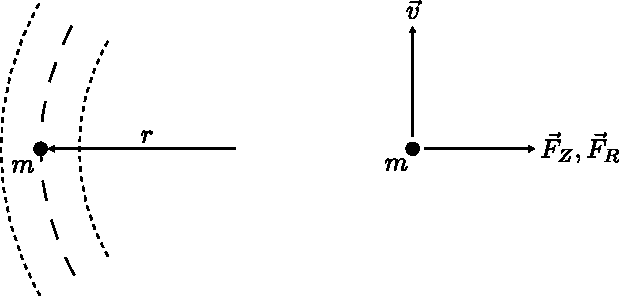
\includegraphics[scale=0.8]{kurve3.pdf}
	\caption{Einfache Kurvenfahrt aus der Vogelperspektive.}
	\label{fig:kurvenfahrt}
\end{figure}

\noindent
Aus der Kreibewegung geht hervor, dass es eine nach innen gerichtete
Kraft $\vec{F}_Z$ mit der entsprechenden Beschleunigung $\vec{a}_{rad}$
gibt. Die Grafik \ref{fig:kurvenfahrt} verdeutlicht, dass im Beispiel 
eines Autos welches durch eine Kurve fährt, diese nach innen gerichtete 
Kraft ebenfalls vorhanden ist. Da bei einem Auto die Reifen eine Reibung 
stellen, muss die Richtung dieser Kraft zwar in der selben Wirkungslinie
sein wie $\vec{F}_Z$, nicht aber die selbe Richtung besitzen.  

\newpage
\section{Steilkurvenfahrt}
Bei einer Steilkurve ist die Höhe des Innen- und Aussenradius nicht
gleich. Eine Betrachtung zu einem bestimmten Punkt in der Kurve stellt
somit eine Kombination aus Hang- und Kreisbewegung dar. 

\begin{figure}[h!]
	\centering
	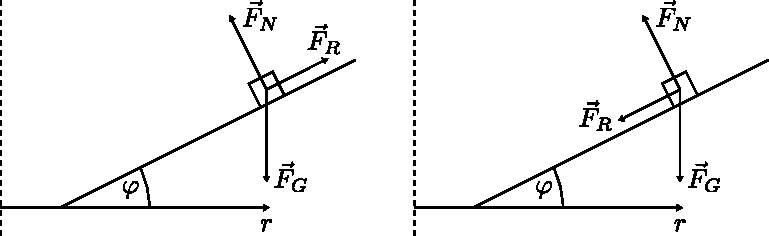
\includegraphics[scale=0.8]{kurve1.pdf}
	\caption{Steilkurve mit 
		$\vec{v}_{klein}$ (l) und $\vec{v}_{gross}$ (r)}
	\label{fig:steilkurve1}
\end{figure}

\noindent
Hierbei gilt es zu beachten, dass die Normalkraft $\vec{F}_N$ nicht 
eine Komponente der Gewichtskraft $\vec{F}_G$ ist, d.h. 
$\vec{F}_N \neq \vec{F}_G \cdot cos(\alpha)$. 

Eine solche Steilkurvenfahrt wird grundsätzlich komponentenweise
betrachtet. Hierzu werden die Kräfte $\vec{F}_N$ und $\vec{F}_R$ in
eine $x$- und $y$-Komponente zerlegt.

\begin{figure}[h!]
	\centering
	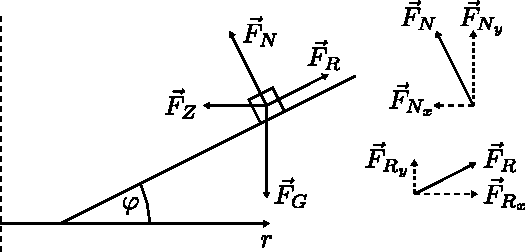
\includegraphics[scale=0.8]{kurve2.pdf}
	\caption{Steilkurve mit zerlegten Kräften in $x,y$}
	\label{fig:steilkurve2}
\end{figure}

\noindent
Sind die Kräfte zerlegt, so können die Bewegungsgleichungen für die 
jeweilige Komponente $x,y$ formuliert werden. Die Vorzeichen sind 
wiederum nach der gewählten Bewegungsrichtung zu setzen. 

\subsection{Lösungsvorgehen}
Um ein Steilkurvenproblem wie im Bild \ref{fig:steilkurve2} dargestellt
zu lösen, kann die folgende Methode angewandt werden.

\begin{enumerate}
	\item Qualitative Skizze erstellen mit allen relevanten Kräften
		des Systems (z.B. $\vec{F}_G$, $\vec{F}_N$, $\vec{F}_R$, 
		$\vec{F}_Z$).
	\item Die winkelabhängigen Kräfte (z.B. $\vec{F}_N, \vec{F}_R$) 
		in $x,y$-Komponenten zerlegen.
	\item Bewegungsrichtung definieren (welche Kraft ist positiv, 
		welche negativ).
	\item Bewegungsgleichung aufstellen für $x,y$
\[\begin{array}{l r c l}
	x: &
		+ \vec{F}_{N_x} - \vec{F}_{R_x} &=& + \vec{F}_Z \\
	& & & \\
	y: &
		+ \vec{F}_{N_y} + \vec{F}_{R_y} &=& + \vec{F}_G
\end{array} \]

	\item Die Kraft, welche zur Kurve normal ist ermitteln (falls
		$\vec{a}_y=0$, dann kann $\vec{F}_N$ durch die
		Bewegungsgleichung von $y$ ermittelt werden).
	\item Restliche Unbekannten ermitteln.
\end{enumerate}
